\ifx\allfiles\undefined

	% 如果有这一部分另外的package,在这里加上
	% 没有的话不需要
	
	\begin{document}
\else
\fi
    \chapter{动态规划}
    目前已介绍的线性规划、运输规划、整数规划、目标规划问题中,没有时间概念。\\
    动态规划是解决多阶段最优决策过程的方法,20世纪50年代由美国数学家贝尔曼等创立。\\
    动态规划基于著名的“最优性原理”,根据多阶段决策问题的特点,把多阶段决策问题变换为\textcolor{red}{一系列互相联系的单阶段问题},然后逐个加以解决。\\
    \section{动态规划问题}

	\textbf{动态规划的本质:}\\
	值得注意的是,动态规划是求解多阶段最优决策问题的一种\textcolor{red}{思想和方法},是分析问题、解决问题的一种途径,而\textcolor{red}{不是一种特殊算法}:
	\begin{itemize}
		\item 单纯形法是一种算法
		\item 最速下降法也是一种算法
	\end{itemize}
		因而,它不像线性规划、非线性规划那样有一个标准的数学表达式和明确定义的一组规则,而必须对具体问题进行具体分析处理,应以丰富的想像力去建立模型,用创造性的技巧去求解。
\\\\\textbf{动态规划问题的分类:}\\根据多阶段决策过程的时间参量是离散的还是连续的变量,过程分为离散决策过程和连续决策过程;根据决策过程的演变是确定性的还是随机性的,过程又可分为确定性决策过程和随机性决策过程。
组合起来就有四种:
\begin{enumerate}
	\item 离散确定性
	\item 离散随机性
	\item 连续确定性
	\item 连续随机性
\end{enumerate}
\textbf{多阶段问题举例:}
可以看一个多阶段问题的例子:
\begin{exbox}{最短路线问题}{}
	\textbf{例:}如图,给定一个线路网络,两点之间连线上的数字表示两点间的距离(或费用),试求一条由A到G的铺管线路,使总距离为最短(或总费用最小)。
	\label{eg:7.1.1}
	\begin{figure}[H]
        \centering
        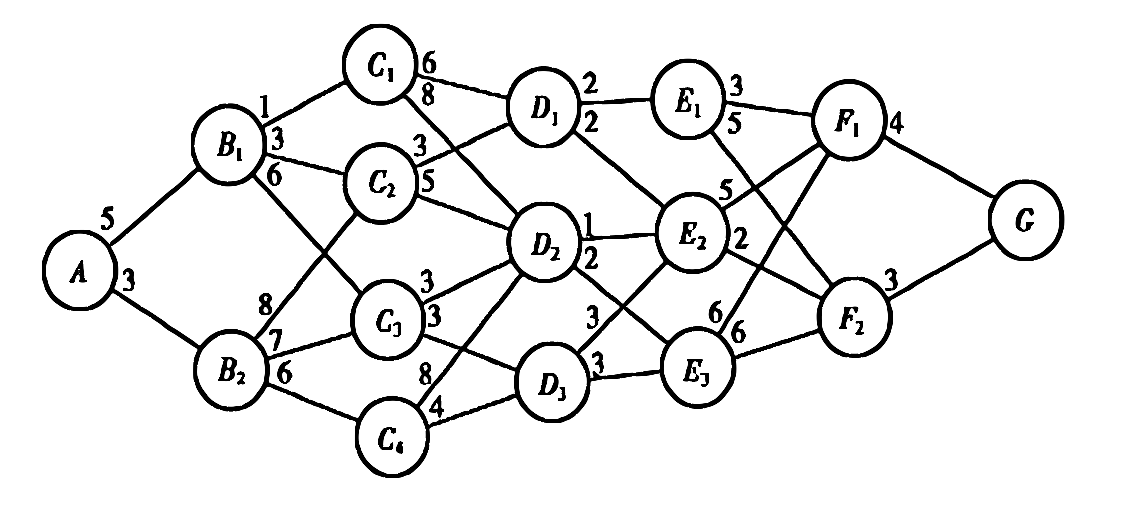
\includegraphics[width=0.8\textwidth]{./image/29.png}
        \caption{路线图}
        \label{fig:Chapter4_Temporary_Pavilion_1}
    \end{figure}
\end{exbox}
    \section{动态规划的基本概念和定义}
	接下来我们给出一些基本概念和定义,其中1-6描述的是约束条件,7描述的是目标函数。
	\begin{enumerate}
	\item{\textbf{多阶段决策过程(序贯决策过程)}}
	\begin{dfnbox}{多阶段决策过程}{}
	把一个问题可看作是前后关联、具有链状结构的多阶段过程,并对其进行决策即\textbf{多阶段决策过程}。
	\end{dfnbox}
	\begin{figure}[H]
        \centering
        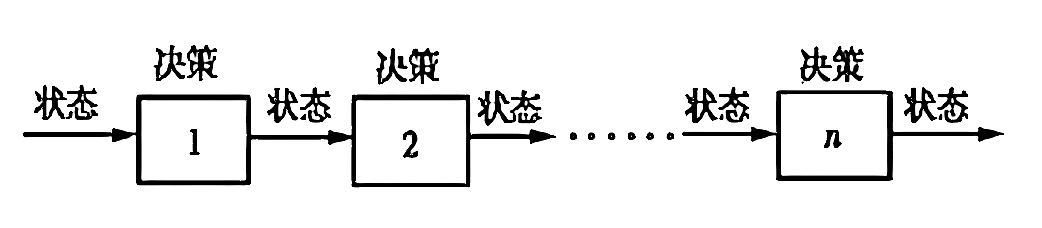
\includegraphics[width=0.6\textwidth]{./image/30.png}
        \caption{多阶段决策过程}
        \label{fig:Chapter4_Temporary_Pavilion_1}
    \end{figure}
在多阶段决策问题中,各个阶段采取的决策一般与时间有关,故有\textcolor{red}{“动态”}的含义。

但是,一些与时间没有关系的静态规划(如线性规划、非线性规划等)问题,只要\textcolor{red}{人为地引进"时间"因素},也可把它视为多阶段决策问题,用动态规划方法去处理。

\item{\textbf{阶段}}
\begin{dfnbox}{阶段}{}
	把过程恰当地分为若干个相互联系的\textbf{阶段},以便能按一定的次序去求解。描述阶段的变量称为\textbf{阶段变量},常用 \( k \) 表示。
\end{dfnbox}
\begin{exbox}{最短路线问题}{}
如\hyperref[eg:7.1.1]{例7.1.1}可分为6个阶段来求解,\( k \) 分别等于1、2、3、4、5、6。
\end{exbox}
\item{\textbf{状态}}
\begin{dfnbox}{状态}{}
	\textbf{状态}表示\textcolor{red}{每个阶段开始}所处的自然状况或客观条件,它描述了研究问题过程的状况。
\end{dfnbox}

\begin{exbox}{最短路线问题}{}
\hyperref[eg:7.1.1]{例7.1.1}中,状态就是某阶段的出发位置。它既是该阶段某支路的起点,又是前一阶段某支路的终点。
通常一个阶段有若干个状态,\hyperref[eg:7.1.1]{例7.1.1}中第一阶段有一个状态,就是点A,第二阶段有两个状态,即点集合 \(\{B_1, B_2\}\),一般第\( k \)阶段的状态就是第\( k \)阶段所有始点的集合。
描述过程状态的变量称为状态变量,常用 \( S_k \) 表示第 \( k \) 阶段的状态变量。
\hyperref[eg:7.1.1]{例7.1.1}中第三阶段有四个状态,则状态变量 \( S_k \) 可取四个值,即 \( C_1 \)、\( C_2 \)、\( C_3 \)、\( C_4 \)。
点集合 \(\{C_1, C_2, C_3, C_4\}\) 就称为第三阶段的可达状态集合。记为 \( S_3 = \{C_1, C_2, C_3, C_4\} \)。
第 \( k \) 阶段的可达状态集合就记为 \( S_k \)。
\end{exbox}

\begin{dfnbox}{状态的性质:无后效性}{}
	\label{dfn:无后效性}
	如果某阶段状态给定后,则在这阶段以后过程的发展不受这阶段以前各段状态的影响。
换句话说,过程的过去历史只能通过当前的状态去影响它未来的发展,当前的状态是以往历史的一个完整总结。
这个性质称为\textbf{无后效性(即马尔科夫性)}。不满足无后效性要求的量不能作为动态规划的状态。
\end{dfnbox}



\item{\textbf{决策}}
\begin{dfnbox}{决策、决策变量、允许决策集合}{}
	\label{允许决策集合}
	\textbf{决策}表示当过程处于某一阶段的某个状态时,可以作出的某种决定(或选择),从而确定下一阶段的状态,这种决定称为决策(在最优控制中也称为控制)。
\\描述决策的变量称为\textbf{决策变量},用 \( u_k(s_k) \) 表示第 \( k \) 阶段当状态处于 \( s_k \) 时的决策变量,它是状态变量的函数。
\\在实际问题中,决策变量的取值往往限制在某一范围之内,此范围称为\textbf{允许决策集合},常用 \( D_k(s_k) \) 表示第 \( k \) 阶段从状态 \( s_k \) 出发的允许决策集合,\( u_k(s_k) \in D_k(s_k) \)。
\end{dfnbox}
每个阶段的决策对于当前阶段未必是最优的,服务于总目标。
\begin{exbox}{最短路线问题}{}
如在\hyperref[eg:7.1.1]{例7.1.1}第二阶段中,若从状态 \( B_1 \) 出发,就可作出三种不同的决策,其允许决策集合
\[ D_2(B_1) = \{C_1, C_2, C_3\}. \]

若选取的点为 \( C_2 \),则 \( C_2 \) 是状态 \( B_1 \) 在决策 \( u_2(B_1) \) 作用下的一个新状态,记作
\[ u_2(B_1) = C_2. \]
\end{exbox}

\item{\textbf{策略}}
\begin{dfnbox}{策略}{}
	\textbf{策略}是一个按顺序排列的决策组成的集合。
\end{dfnbox}
\begin{dfnbox}{后部子过程}{}
	由过程的第 \( k \) 阶段开始到终止状态为止的过程,称为问题的\textbf{后部子过程}(或称为 \( k \) 子过程)。
\end{dfnbox}
\begin{dfnbox}{k子过程策略}{}
	由每段的决策按顺序排列组成的决策函数序列 \(\{u_k(s_k), u_{k+1}(s_{k+1}), \cdots, u_n(s_n)\}\) 称为
	\textbf{\( k \) 子过程策略},简称\textbf{子策略},记为 \( p_{k,n}(s_k) \)。即:
\[ p_{k,n}(s_k) = \{u_k(s_k), u_{k+1}(s_{k+1}), \cdots, u_n(s_n)\}. \]
\\特别地,当 \( k = 1 \) 时,此决策函数序列称为\textbf{全过程的一个策略},简称\textbf{策略},记为 \( P_{1,n}(s_1) \)。即,
\[ P_{1,n}(s_1) = \{u_1(s_1), u_2(s_2), \ldots, u_n(s_n)\}. \]
\end{dfnbox}
实际问题中,可供选择的策略有一定的范围,此范围称为允许\textcolor{red}{策略集合},用 \( P \) 表示。
从允许策略集合中找出达到最优效果的策略称为\textcolor{red}{最优策略}。

\item {\textbf{状态转移方程}}
\begin{dfnbox}{状态转移方程}{}
	\label{dfn:状态转移方程}
	\textbf{状态转移方程}是确定过程由一个状态到另一个状态的演变过程。
\end{dfnbox}
\begin{thmbox}{状态转移方程}{}
若给定第 \( k \) 阶段状态变量 \( S_k \) 的值,如果该段的决策变量 \( u_k \) 一经确定,第 \( k+1 \) 阶段的状态变量 \( S_{k+1} \) 的值也就完全确定,即 \( S_{k+1} \) 的值随 \( S_k \) 和 \( u_k \) 的值变化而变化,这种确定的对应关系,记为
\[S_{k+1} = T_k (S_k, u_k).\]

上式描述了由 \( k \) 阶段到 \( k+1 \) 阶段的状态转移规律,称为状态转移方程。\( T_k \) 称为状态转移函数。
\end{thmbox}
\begin{exbox}{最短路线问题}{}
\hyperref[eg:7.1.1]{例7.1.1}中,状态转移方程为 \( S_{k+1} = u_k (S_k) \)。
\end{exbox}
\item \textbf{指标函数和最优值函数}
\begin{dfnbox}{指标函数}{}
用来衡量所实现过程优劣的一种数量指标,称为\textbf{指标函数}。它是定义在全过程和所有后部子过程上确定的数量函数。常用 \( V_{k,n} \) 表示,即:
\[V_{k,n} = V_{k,n}(s_k, u_k, s_{k+1}, u_{k+1}, \cdots, s_{n+1}), \, k = 1, 2, \cdots, n.\]
\end{dfnbox}
\begin{thmbox}{动态规划指标函数的要求}{}
对于要构成动态规划模型的指标函数应满足两个条件:
\begin{itemize}
\item 具有\textcolor{red}{可分离性}
\item 满足\textcolor{red}{递推关系}\footnote{换句话说,总是构成新的一阶段的指标函数是由历史上所有阶段的指标函数与当前阶段的指标函数做某种运算 (包括但不限于加、减、乘、除...)},即 \( V_{k,n} \) 可以表示为 \( s_k, u_k, V_{k+1,n} \) 的函数。记为:
\[V_{k,n}(s_k, u_k, s_{k+1}, u_{k+1}, \cdots, s_{n+1}) = \psi(s_k, u_k, V_{k+1,n}(s_{k+1}, u_{k+1}, \cdots, s_{n+1})).\]
简记为 \( V_{k,n} = \psi(s_k, u_k, V_{k+1,n}). \)
\end{itemize}
\end{thmbox}
我们可以注意到,在这个指标函数中,真正独立的变量只有\textcolor{red}{初始状态$s_0$以及所有$u_k$},其他状态都是被这些量唯一确定的,并不独立。
\\\\\textbf{常见的指标函数:}\\
有\textcolor{red}{加和乘}两种:
\begin{enumerate}[label=(\arabic*)]
    \item 过程和它的任一子过程的指标是它所包含的各阶段的指标的和。即
    \[V_{k,n}(S_k, t_k, \cdots, S_{n+1}) = \sum_{j=k}^{n} v_j(S_j, t_j)\]
    这时,
    \[V_{k,n}(S_k, t_k, \cdots, S_{n+1}) = v_k(S_k, t_k) + V_{k+1,n}(S_{k+1}, t_{k+1}, \cdots, S_{n+1})\]
    
    \item 过程和它的任一子过程的指标是它所包含的各阶段的指标的乘积。即
    \[V_{k,n}(S_k, t_k, \cdots, S_{n+1}) = \prod_{j=k}^{n} v_j(S_j, t_j)\]
    这时,
    \[V_{k,n}(S_k, t_k, \cdots, S_{n+1}) = v_k(S_k, t_k) V_{k+1,n}(S_{k+1}, t_{k+1}, \cdots, S_{n+1})\]
\end{enumerate}
\begin{dfnbox}{最优值函数}{}
指标函数的最优值,称为\textbf{最优值函数},记为 \( f_k(s_k) \)。它表示从第k阶段的状态 \( s_k \) 开始到第n阶段的终止状态的过程,当采取最优策略时所得到的指标函数数值。即:
\[f_k(S_k) = \text{opt} \{ u_k, \cdots, u_n \}\]\footnote{其中"opt"可根据题意而取min或max。}
\end{dfnbox}
在不同的问题中,指标函数的含义是不同的,可能是距离、利润、成本、产品的产量或资源消耗等。
\begin{exbox}{最短路线问题}{}
\hyperref[eg:7.1.1]{例7.1.1}中,指标函数 \( V_{k,n} \) 就表示在第 \( k \) 阶段由点 \( s_k \) 至终点 \( G \) 的距离。用
\[d_k(s_k, u_k) = v_k(s_k, u_k).\]
表示在第 \( k \) 阶段由点 \( s_k \) 到点 \( s_{k+1} = u_k(s_k) \) 的距离。
\end{exbox}
\end{enumerate}


\section{动态规划求解方法}
\subsection{逆序方法}
我们仍然以\hyperref[eg:7.1.1]{例7.1.1}为例,对于像这样的最短路问题,有一个重要性质:
\begin{thmbox}{最优性原理}{}
如果由起点A经过P点和H点而到达终点G是一条最短路线,则由点P出发经过H点到达终点G的这条子路线,对于从点P出发到达终点的所有可能选择的不同路线来说,必定也是最短路线。
\\此性质可由反证法来证明。
\end{thmbox}
寻找\hyperref[eg:7.1.1]{例7.1.1}最短路线的方法,可以考虑从最后一段开始,用由后向前逐步递推的方法,求出各点到G点的最短路线,最后求得由A点到G点的最短路线。
\begin{dfnbox}{逆序方法}{}
	动态规划中这种从终点逐段向始点方向寻找最短路线的策略称为\textbf{逆序方法}
\end{dfnbox}
\begin{exbox}{最短路线问题}{}
	\begin{figure}[H]
        \centering
        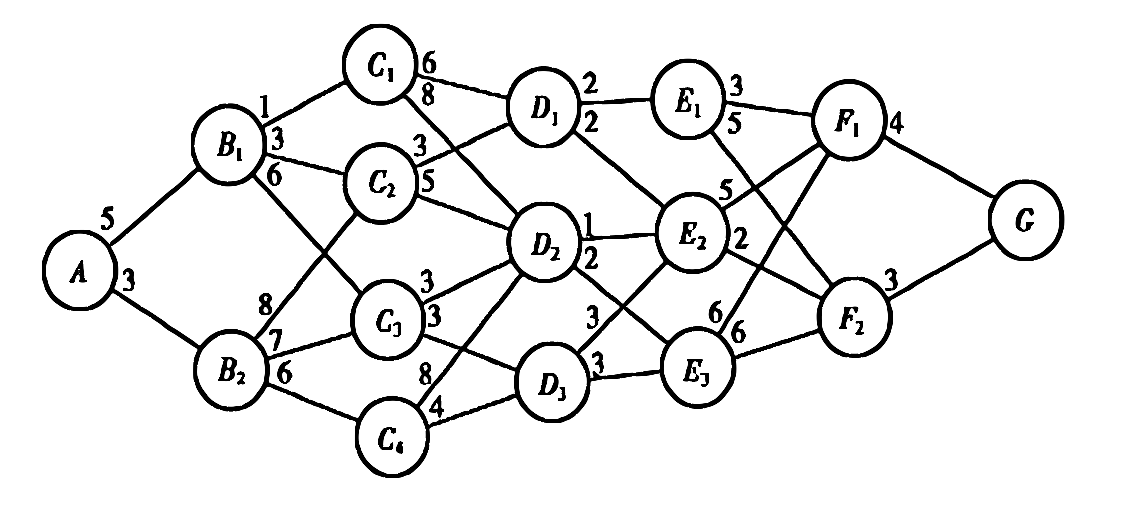
\includegraphics[width=0.8\textwidth]{./image/29.png}
        \caption{路线图}
        \label{fig:Chapter4_Temporary_Pavilion_1}
    \end{figure}
	从最后一段开始计算,由后向前逐步推移至A点。
	当 \( k = 6 \) 时,由 \( F_1 \) 到终点 \( G \) 只有一条路线,故 \( f_6(F_1) = 4 \)。同理,\( f_6(F_2) = 3 \)。
	当 \( k = 5 \) 时,出发点有 \( E_1, E_2, E_3 \) 三个。若从 \( E_1 \) 出发,则有两个选择:a.至 \( F_1 \);b.至 \( F_2 \)
		\\则
		\[f_5(E_1) = \min 
		\begin{cases} 
		d_5(E_1, F_1) + f_6(F_1) \\
		d_5(E_1, F_2) + f_6(F_2)
		\end{cases}
		= \min
		\begin{cases} 
		3 + 4 \\
		5 + 3
		\end{cases}
		= 7\]
		其相应的决策为 \( u_5(E_1) = F_1 \)
		
		这说明,由 \( E_1 \) 至终点 \( G \) 的最短距离为7,其最短路线是  
		\[E_1 \rightarrow F_1 \rightarrow G\]  
		
		同理,从 \( E_2 \) 和 \( E_3 \) 出发,则有  
		\[f_5(E_2) = \min \left\{ \begin{array}{l} 
		d_5(E_2, F_1) + f_6(F_1) \\ 
		d_5(E_2, F_2) + f_6(F_2) 
		\end{array} \right\} = \min \left\{ \begin{array}{l} 
		5 + 4 \\ 
		2 + 3 
		\end{array} \right\} = 5\]  
		其相应的决策为  
		\[u_5(E_2) = F_2\]  
		\[f_5(E_3) = \min \left\{ \begin{array}{l} 
		d_5(E_3, F_1) + f_6(F_1) \\ 
		d_5(E_3, F_2) + f_6(F_2) 
		\end{array} \right\} = \min \left\{ \begin{array}{l} 
		6 + 4 \\ 
		6 + 3 
		\end{array} \right\} = 9\]  
		且  
		\[u_5(E_3) = F_2\]
		
		类似地,可算得:  
		当 \( k = 4 \) 时,有  
		\[f_4(D_1) = 7 \quad u_4(D_1) = E_2\]  
		\[f_4(D_2) = 6 \quad u_4(D_2) = E_2\]  
		\[f_4(D_3) = 8 \quad u_4(D_3) = E_2\]  
		
		当 \( k = 3 \) 时,有  
		\[f_3(C_1) = 13 \quad u_3(C_1) = D_1\]  
		\[f_3(C_2) = 10 \quad u_3(C_2) = D_1\]  
		\[f_3(C_3) = 9 \quad u_3(C_3) = D_2\]  
		\[f_3(C_4) = 12 \quad u_3(C_4) = D_3\]
		
		当 \( k = 2 \) 时,有
		\[f_2(B_1) = 13 \quad u_2(B_1) = C_1\]
		\[f_2(B_2) = 16 \quad u_2(B_2) = C_2\]
		
		当 \( k = 1 \) 时,出发点只有一个 \( A \) 点,则
		\[f_1(A) = \min \left\{ 
		\begin{array}{l}
		d_1(A, B_1) + f_2(B_1) \\
		d_1(A, B_2) + f_2(B_2)
		\end{array} 
		\right\} = \min \left\{ 
		\begin{array}{l}
		5 + 13 \\
		3 + 16
		\end{array} 
		\right\} = 18\]
		且 \( u_1(A) = B_1 \)。于是得到从起点 \( A \) 到终点 \( G \) 的最短距离为18。
		
		为了找出最短路线,再按计算的顺序反推之,可求出最优决策函数序列 \(\{u_k\}\),即由  
		\[ u_1(A) = B_1, u_2(B_1) = C_1, u_3(C_1) = D_1, u_4(D_1) = E_2, u_5(E_2) = F_2, u_6(F_2) = G \]  
		组成一个最优策略。因此,找出相应的最短路线为  
		\[ A \rightarrow B_1 \rightarrow C_1 \rightarrow D_1 \rightarrow E_2 \rightarrow F_2 \rightarrow G \]
		\begin{figure}[H]
			\centering
			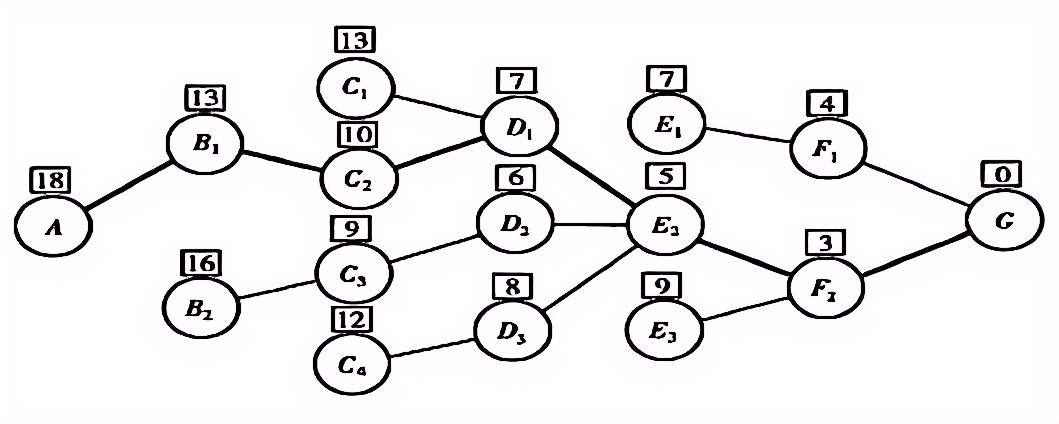
\includegraphics[width=0.8\textwidth]{./image/31.png}
			\caption{逆序求解路线,数字代表每一个状态点到终点G的最优路径}
			\label{fig:Chapter4_Temporary_Pavilion_1}
		\end{figure}
\end{exbox}
上面的计算过程中表明,在求解的各个阶段,利用了 \( k \) 阶段与 \( k+1 \) 阶段之间的如下递推关系:
		\[\begin{cases} 
		f_k(s_k) = \min_{u_k \in D_k(s_k)} \{ d_k(s_k, u_k(s_k)) + f_{k+1}(u_k(s_k)) \} \quad k = 6, 5, 4, 3, 2, 1 \\ 
		f_7(s_7) = 0 \quad (\text{或写成 } f_6(s_6) = d_6(s_6, G))
		\end{cases}\]
	\begin{thmbox}{动态规划逆序方法的基本方程}{}
		一般情况,k 阶段与 \( k+1 \) 阶段的递推关系式
		\[f_k(S_k) = \text{opt}_{u_k \in D_k(S_k)} \left\{ v_k(S_k, u_k(S_k)) + f_{k+1}(u_k(S_k)) \right\}\]
		\[k = n, n-1, \cdots, 1\]
		边界条件\footnote{为什么要有边界条件呢?这就相当于微分方程、差分方程中用以解待定系数的“初值”,本质上是因为我们分阶段的过程类似于微分方程、差分方程的过程,因为他们都有“过程”的概念,体现了来自过去的信息、动态的信息}为
		\[f_{n+1}(S_{n+1}) = 0\]
	\end{thmbox}
\subsection{顺序方法}
\hyperref[eg:7.1.1]{例7.1.1}中,由于线路网络的两端都是固定的,且线路上的数字是表示两点间的距离,则从A点计算到G点和从G点计算到A点的最短路线是相同的。因而,求解过程也可以由A开始,从前向后展开,只不过此时视G 为起点,A为终点。
这种以G为始端、A为终端的从A到G的解法称为\textbf{顺序方法}。\\
忽略顺序方法的具体求解过程,其结果如下图
\begin{figure}[H]
	\centering
	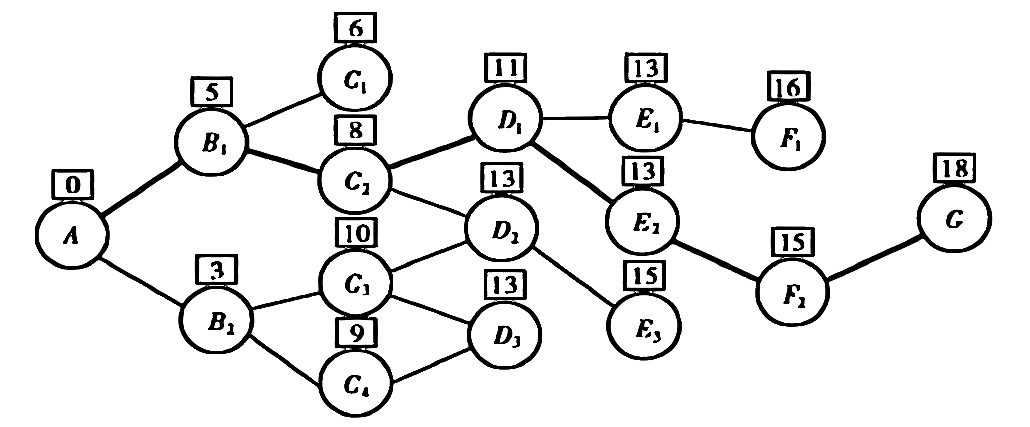
\includegraphics[width=0.8\textwidth]{./image/32.png}
	\caption{顺序求解路线,数字代表每一个状态点到起点A的最优路径}
	\label{fig:Chapter4_Temporary_Pavilion_1}
\end{figure}

\begin{notebox}{\textbf{结论}}{}
	\\\textcolor{red}{起点定了用顺序法,终点定了用逆序法。}
\end{notebox}
\section{动态规划基本方程的建立与最优性原理}
动态规划基本方程
\begin{thmbox}{逆序方法的基本方程的推导}{}
	对于逆序方法,设指标函数是取各阶段指标的\textcolor{red}{和}的形式,即  
	\[V_{k,n} = \sum_{j=k}^{n} v_j (s_j, u_j)\]
	其中 \(v_j (s_j, u_j)\) 表示第 \(j\) 段的指标。
	
	显然满足指标函数的可分离性,所以上式可写成
	\[V_{k,n} = v_k (s_k, u_k) + V_{k+1,n} [s_{k+1}, \cdots, s_{n+1}]\footnote{称之为“一串加一步”的方式,“一串”是k+1到n,“一步”是k到k+1}\]
	
	当初始状态给定时,过程的策略就被确定,则指标函数也就确定了。因此,指标函数是\textcolor{red}{初始状态和策略}的函数。可记为 \(V_{k,n}[s_k, p_{k,n}(s_k)]\) 故上面递推关系又可写成
	\[V_{k,n}[s_k, p_{k,n}] = v_k(s_k, u_k) + V_{k+1,n}[s_{k+1}, p_{k+1,n}]\]
	其子策略 \(p_{k,n}(s_k)\) 可看成是由决策 \(u_k(s_k)\) 和 \(p_{k+1,n}(s_{k+1})\) 组合而成。即
	\[p_{k,n} = \{u_k(s_k), p_{k+1,n}(s_{k+1})\}\]
	
	如果用 \( p_{k,n}^*(s_k) \) 表示初始状态为 \( s_k \) 的后部子过程所有子策略中的最优子策略,则最优值函数为
	\[f_k(s_k) = V_{k,n}[s_k, p_{k,n}^*(s_k)] = \text{opt} V_{k,n}[s_k, p_{k,n}(s_k)]\]
	
	而
	\[
	\begin{aligned}
	\text{opt} V_{k,n}(s_k, p_{k,n}) &= \text{opt}_{\{u_k, p_{k+1,n}\}} \{v_k(s_k, u_k) + V_{k+1,n}(s_{k+1}, p_{k+1,n})\} \\
	&= \text{opt}_{u_k}\{v_k(s_k, u_k) + \text{opt}_{p_{k+1,n}} V_{k+1,n}(s_{k+1}, p_{k+1,n})\footnote{“一步”加上“最优的一串”再取最优}\}
	\end{aligned}
	\]
\end{thmbox}
	
	\begin{notebox}{\textbf{动态规划基本方程的求解过程}}
	\\根据边界条件,从 \( k = n \) 开始,由后向前逆推,从而逐步可求得各段的最优决策和相应的最优值,最后求出 \( f_1 (s_1) \) 时,就得到整个问题的最优解。
	\end{notebox}

	\begin{notebox}{\textbf{动态规划基本方程的建立原则}}
		\\
	给一个实际问题建立动态规划模型时,必须做到下面五点:
	\begin{enumerate}[label=(\arabic*)]
		\item 将问题的过程划分成恰当的阶段
		
		\item 正确选择状态变量 \( s_k \),使它既能描述过程的演变,又要满足\hyperref[dfn:无后效性]{无后效性}。
		
		\item 确定决策变量 \( u_k \) 及每阶段的\hyperref[允许决策集合]{允许决策集合} \( D_k(s_k) \)
		
		\item 正确写出\hyperref[dfn:状态转移方程]{状态转移方程}
	
		\item 正确写出指标函数 \( V_{k,n} \) 的关系,它应满足下面三个性质:
		\begin{enumerate}[label=\roman*.]
			\item 是定义在全过程和所有后部子过程上的数量函数
			
			\item 要具有可分离性,并满足递推关系。即,
			\[V_{k,n}(s_k, u_k, \cdots, s_{n+1}) = \psi_k[s_k, u_k, V_{k+1,n}(s_{k+1}, u_{k+1}, \cdots, s_{n+1})]\]
			
			\item 函数 \(\psi_k(s_k, u_k, V_{k+1,n})\) 对于变量 \( V_{k+1,n} \) 要严格单调
		\end{enumerate}
	\end{enumerate}
	以上五点是构造动态规划模型的基础,是正确写出动态规划基本方程的基本要素。
	\\一旦建立了动态规划模型,就可以用逆序或顺序方法进行求解。
\end{notebox}
	

\ifx\allfiles\undefined
	% 如果有这一部分的参考文献的话,在这里加上
	% 没有的话不需要
	% 因此各个部分的参考文献可以分开放置
	% 也可以统一放在主文件末尾。
	
	%  bibfile.bib是放置参考文献的文件,可以用zotero导出。
	% \bibliography{bibfile}
	
	end{document}
	\else
	\fi